\documentclass[11pt, a4paper]{article}
\usepackage{graphicx}
\usepackage{amsmath}
\usepackage{listings}
\usepackage{minted}
\usepackage{graphicx}
\usepackage{amsmath}
\usepackage[margin=0.8in]{geometry}
\usepackage{listings}
\usepackage{float}
\usepackage{fancyhdr}
\usepackage{indentfirst}
\usepackage[inline]{enumitem}
\usepackage{xcolor}
\usepackage{minted}
\usemintedstyle{vs}

\title{Assignment No :6: 1-D Simulation of tube-light} 

\author{Sakthi Harish D T (EE19B054)} 

\date{April $7^{th}$, 2021} 
\begin{document}		
		
\maketitle 
\section{Abstract:}
In this assignment ,we will,
\begin{enumerate}
    \item Simulate a tube-light in One-Dimension 
    \item Visualize the electron population density and intensity at every point along the length of the tube light
    \item Print the values of intensity along the length of the tube-light.
    \item compare the graphs obtained for some other values of threshold velocity and probability of collision.
\end{enumerate}

\section{Introduction:}
In a tube-light, the electrons originate from the cathode and move towards the anode due to the applied electric potential. The electric field that has been setup due to the applied potential in between ends of the tube light accelerates the electrons and thus energizes it. Therefore if some electron crosses a threshold energy, then it can excite the atom which it collides and thus it can emit light while de-excitation. But there is some probability with which the electron collides with an atom.
\newline

We create our simulation environment as a array of size 'n', where the tube is divided into 'n' sections. In each time instant, 'M' electrons are injected into the environment. We run the simulation for 'nk' turns. The electrons are unable to excite the atoms till they posses a threshold velocity of 'u0'. Beyond this velocity, there is a probability 'p' in each turn that a collision will occur and an atom gets excited. The electron’s velocity reduces to zero if it collides(inelastic). Here the parameters discussed are taken from the user (\texttt{sys.argv}), along with a set of default values.

\section{Initializing Vectors:}
We create vectors of size 'n*M' to hold the information of the electrons and initialize them to zero, this includes 
\begin{enumerate}
    \item Electron position (xx)
    \item Electron velocity (u)
    \item Displacement in current turn (dx)
\end{enumerate}

In order to accumulate the information gathered in each loop of simulation, we create lists for the following
\begin{enumerate}
    \item Intensity of emitted light(I)
    \item Electron position(X)
    \item Electron velocity(V)
\end{enumerate}

For each turn, we record all electron positions and velocities in these arrays.  If they had a collision, we also record that as emitted light. We do not know the length of these arrays.  So we create them as lists and extend them as required. So, this is a bit slow.

\section{Performing the iteration:}
As mentioned above, we loop 'nk' times and update the electron position, velocity and apply the threshold conditions and update their values and finally retrieve the corresponding Intensity, position and velocity values of the electron along all sections of the tube light.
This is done as per the following code:
    \textit{\textbf{Python Code:}}
    \lstset{language=Python}
    \lstset{label={lst:code_direct}}
    \lstset{basicstyle=\footnotesize}
    \begin{lstlisting}
for k in range(nk-1):
    ii= np.where(xx>0)       #finding the indices of positions greater than zero
    dx[ii]= u[ii]+ 0.5        #Updating the vectors
    xx[ii]= xx[ii]+ dx[ii]     
    u[ii]= u[ii]+ 1           
    
    anode_hit= np.where(xx[ii]>n)     #Finding the indices of electrons that reached anode
    xx[ii[0][anode_hit]]= 0       #Updating the values after hitting the anode
    u[ii[0][anode_hit]]= 0
    dx[ii[0][anode_hit]]= 0

    kk= np.where(u>= u0)       #Finding the indices of energetic electrons
    ll= np.where(np.random.rand(len(kk[0]))<= p)     #Vector of indices, containing indices of kk  
    kl= kk[0][ll]              #Vector of indices of kk np.where collision occurs
    u[kl]= 0               #Updating the velocity of electrons suffering collision

    xx[kl]= xx[kl]- (dx[kl]* np.random.rand(len(kl)))    #randomly deciding np.where the collision took place
    I.extend(xx[kl].tolist())
    m= int(np.random.rand()*Msig)+ M
    
    free= np.where(xx==0)       #Finding free spaces in the grid
    n_inject= min((n*M)-len(free),m)
    
    xx[free[:n_inject]]= 1    #Updating the values of vectors corresponding to the injected electrons
    u[free[0][:n_inject]]= 0   # (i.e) position= 1; velocity= 0 ; displacement= 0
    dx[free[0][:n_inject]]= 0         
    X.extend(xx.tolist())
    V.extend(u.tolist())
    \end{lstlisting}


\section{Plotting the Graphs:}
After we do the iterations, we finally plot the histogram plot of the Population of electrons and the Intensity plot, along with the Electron space phase plot. These are shown in the following figures:
\clearpage

\begin{figure}[!tbh]
\centering
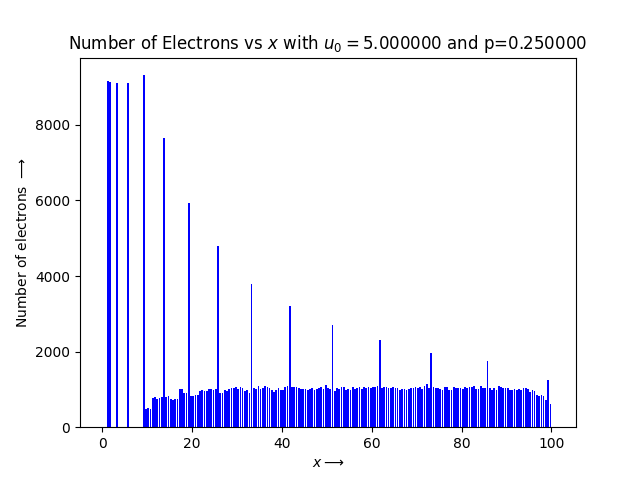
\includegraphics[scale=0.56]{hist1_elec_density.png} 
\caption{Population plot of the electrons}
\label{fig:fig_1}
\end{figure} 

\begin{figure}[!tbh]
\centering
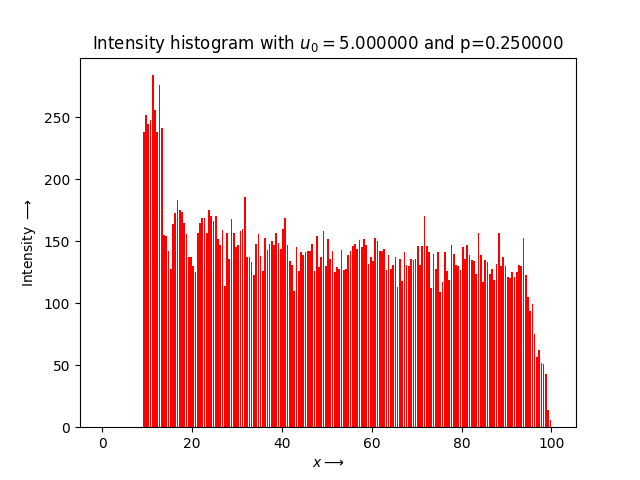
\includegraphics[scale=0.56]{hist1_intensity.png} 
\caption{Intensity plot of the electrons}
\label{fig:fig_2}
\end{figure} 

\begin{figure}[!tbh]
\centering
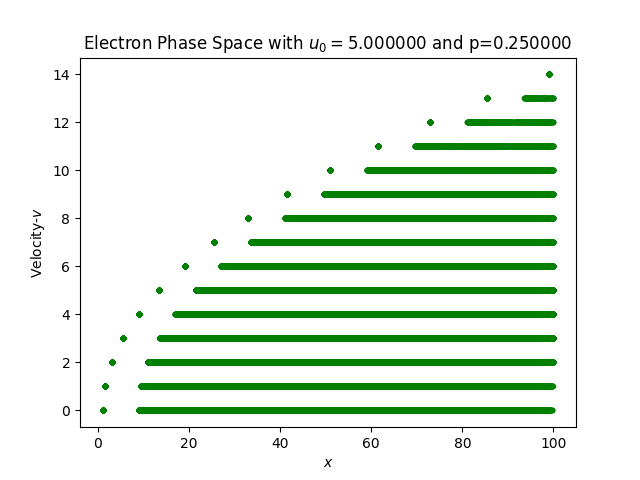
\includegraphics[scale=0.56]{elec_phasa_space.png} 
\caption{Electron space phase plot}
\label{fig:fig_3}
\end{figure} 

We also make a table of the Intensity data against the \texttt{xpos}, this is as shown below:
\begin{verbatim}	
Intensity Data: 
 xpos 	 count 
 
0.25 	 0.000000
0.75 	 0.000000
1.25 	 0.000000
1.75 	 0.000000
2.25 	 0.000000
2.75 	 0.000000
3.25 	 0.000000

..   ...    ...
97.75 	 51.000000
98.25 	 42.000000
98.75 	 29.000000
99.25 	 21.000000
99.75 	 5.000000
100.25 	 0.000000

\end{verbatim}

\section{Analysing with different set of values:}
\begin{enumerate}
    \item In this section we try to vary the parameters that decides the simulation pattern and visualize the same and seek out some inferences from the same.
    \item One specific observation is that as the probability increases the graphs become more variate i.e. the superposition of the probability graphs become more separated. We also see that the maximum intensity also increases as the electrons get ionized more often.
    \item Also as the cutoff velocity is increased the initial excitation happens at a higher value of x. This is because the electron has to travel longer distances to be able to reach cutoff frequency.
\end{enumerate}


\begin{figure}[!tbh]
\centering
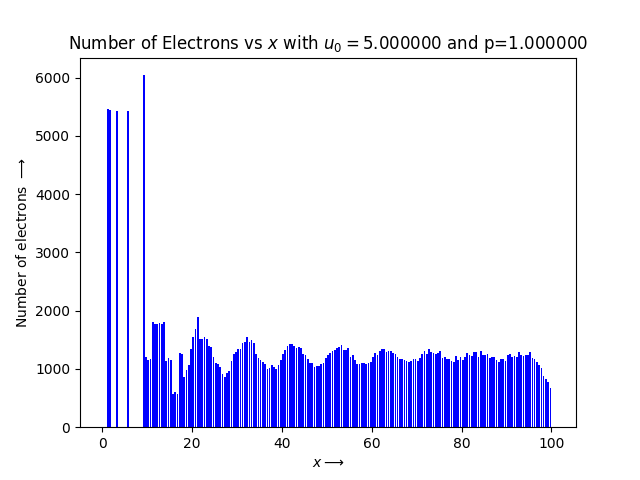
\includegraphics[scale=0.56]{hist2_elec_density.png} 
\caption{Population plot of the electrons}
\label{fig:1fig_1}
\end{figure} 

\begin{figure}[!tbh]
\centering
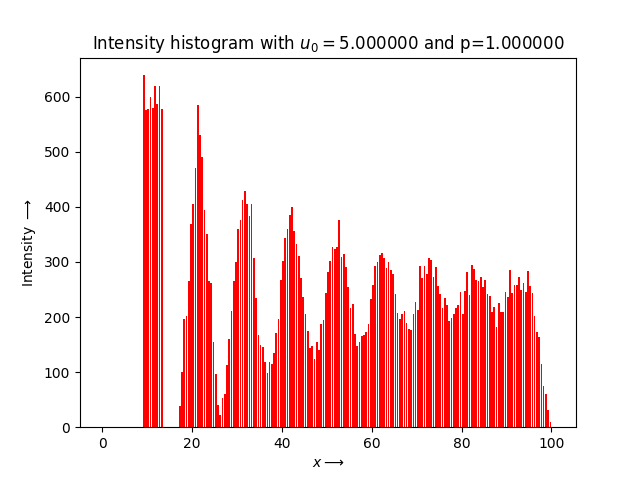
\includegraphics[scale=0.56]{hist2_intensity.png} 
\caption{Intensity plot of the electrons}
\label{fig:1fig_2}
\end{figure} 

\begin{figure}[!tbh]
\centering
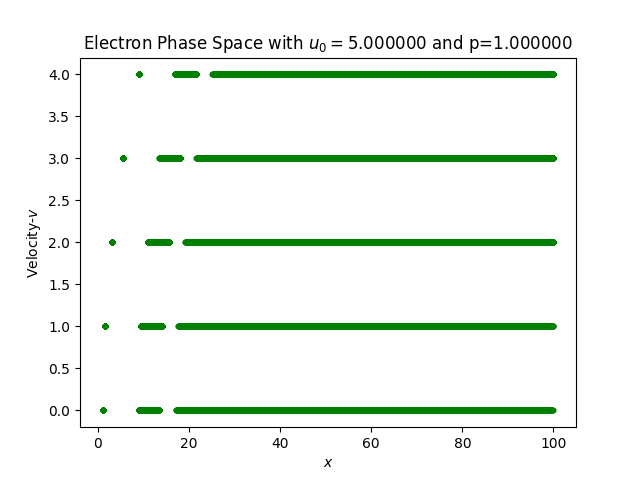
\includegraphics[scale=0.6]{elec_phasa_space2.png} 
\caption{Electron space phase plot}
\label{fig:1fig_3}
\end{figure}

\begin{figure}[!tbh]
\centering
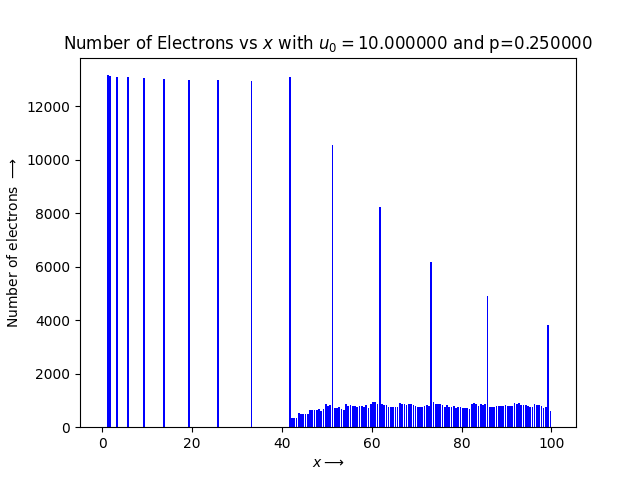
\includegraphics[scale=0.56]{hist3_elec_density.png} 
\caption{Population plot of the electrons}
\label{fig:2fig_1}
\end{figure} 

\begin{figure}[!tbh]
\centering
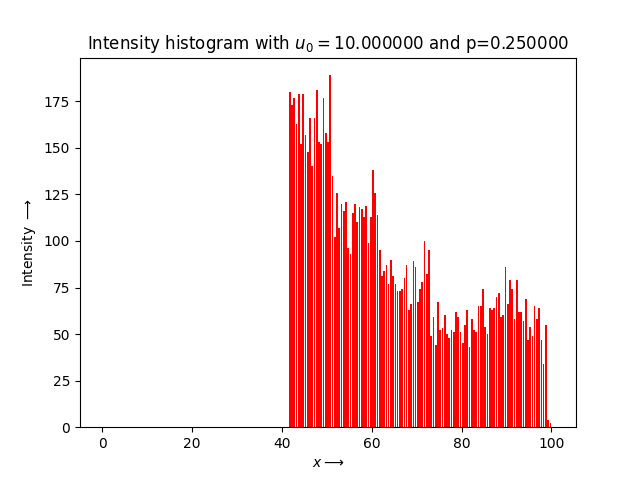
\includegraphics[scale=0.56]{hist3_intensity.png} 
\caption{Intensity plot of the electrons}
\label{fig:2fig_2}
\end{figure} 

\begin{figure}[!tbh]
\centering
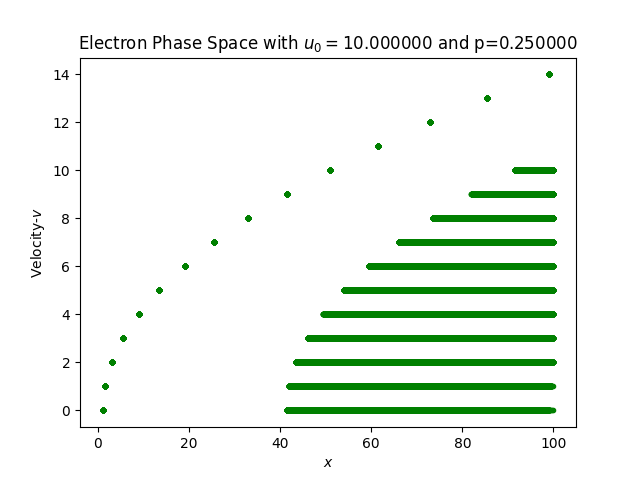
\includegraphics[scale=0.6]{elec_phasa_space3.png} 
\caption{Electron space phase plot}
\label{fig:2fig_3}
\end{figure} 


\begin{figure}[!tbh]
\centering
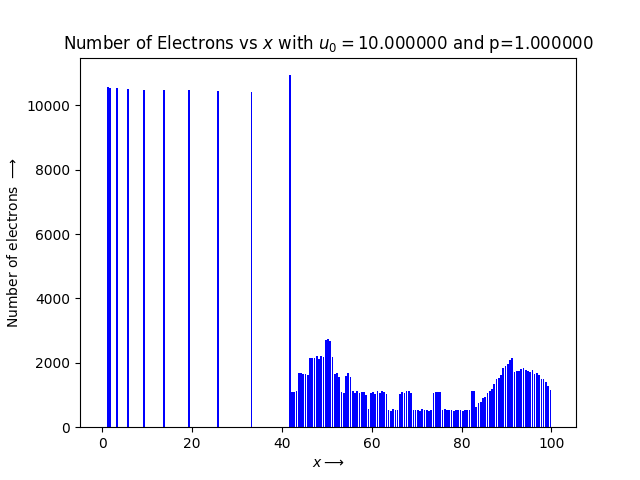
\includegraphics[scale=0.56]{hist4_elec_density.png} 
\caption{Population plot of the electrons}
\label{fig:3fig_1}
\end{figure} 

\begin{figure}[!tbh]
\centering
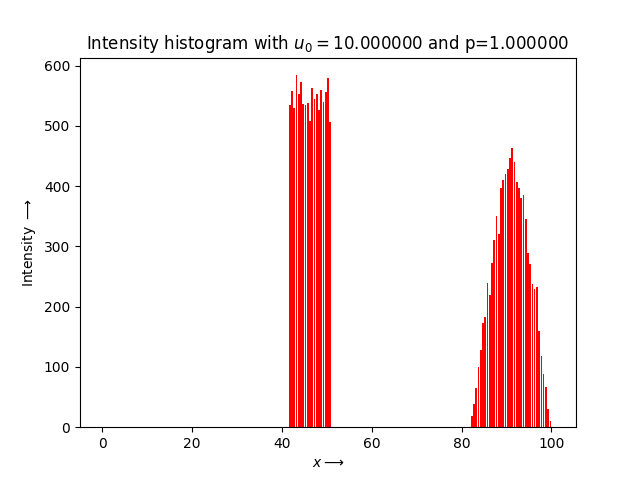
\includegraphics[scale=0.56]{hist4_intensity.png} 
\caption{Intensity plot of the electrons}
\label{fig:3fig_2}
\end{figure} 

\begin{figure}[!tbh]
\centering
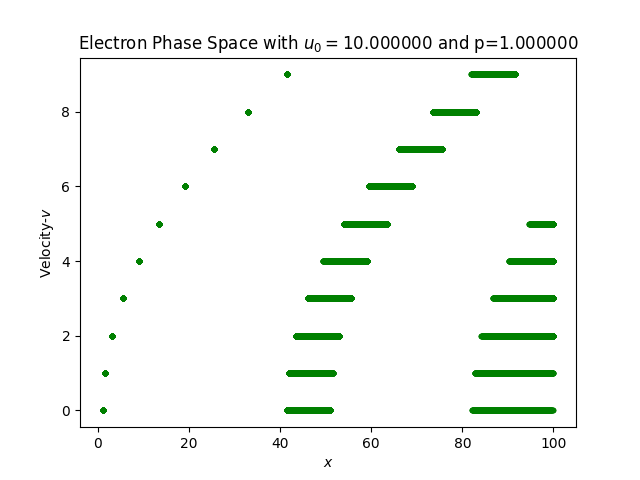
\includegraphics[scale=0.56]{elec_phasa_space4.png} 
\caption{Electron space phase plot}
\label{fig:3fig_3}
\end{figure} 
\newpage
\newline
\newline\newline\newline
\section{Conclusion:}
\begin{enumerate}
    \item From the Intensity plot of the electrons(for p=0.25; $u_0$=5), we see that it reaches a maximum at around x=15 and stays like that for few bins and then it decreases.
    \item This is because of the fact that the electron comes to rest after collision with other atom. So it has to start regaining energy from zero to be able to excite the atom for emitting light.
    \item From the Electron phase space, we see that there are certain specified values of velocity that can occur at a particular value of x, thus we could say that the velocities are quantized.
    \item We have analysed a 1-D tubelight using python and visualized it using histograms. 
\end{enumerate}

\end{document}

 
